\chapter{Aside: floating tables, caption and references}\label{sec:aside}

Before continuing the tutorial (you already saw the essential parts), let's take a few moments to look at how our tables are displayed.

Until now, our tables are directly inserted into the document, exactly at the place in the text where we wrote them. But this can sometimes lead to an unpleasant display, for instance where the table is at the end of a page and there is not enough space, causing an early page break.

Let's take an example:

\begin{Code}
Lorem ipsum dolor sit amet.
% So much more text
Here's the list of my previous trips:

\begin{tblr}{
	colspec = {llX},
	row{1} = {font=\bfseries},
}
	Place & Date & Comment \\ \hline
	Japan & May 2025 & A trip long awaited! I visited everything and ate all the rest. \\
	Castles of the Loire & January 2025 & Very nice to go around by bikes. \\
	Calanques of Marseille & July 2024 & Lots of people. Plan water for your hikes. \\
	Berlin & June 2024 & The weekend would \textit{probably} have been pleasant if our train had not been 8 hours late...\\
\end{tblr}

So many adventures!
\end{Code}

Which could render as:

\begin{center}
	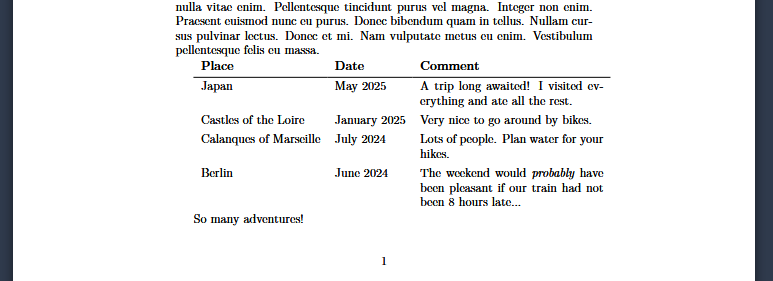
\includegraphics[width=\linewidth]{../img/longtblr_intro}
\end{center}

What if we add a new entry?

\begin{Code}
	Lorem ipsum dolor sit amet.
	% So much more text
	Here's the list of my previous trips:
	
	\begin{tblr}{
		colspec = {llX},
		row{1} = {font=\bfseries},
	}
		Place & Date & Comment \\ \hline
		Japan & May 2025 & A trip long awaited! I visited everything and ate all the rest. \\
		Castles of the Loire & January 2025 & Very nice to go around by bikes. \\
		Calanques of Marseille & July 2024 & Lots of people. Plan water for your hikes. \\
		Berlin & June 2024 & The weekend would \textit{probably} have been pleasant if our train had not been 8 hours late...\\
		Halles Bocuse & April 2014 & Luckily I don't live in Lyon, I would end up overweight and ruined in a matter of days.
	\end{tblr}
	
	So many adventures!
\end{Code}


\begin{center}
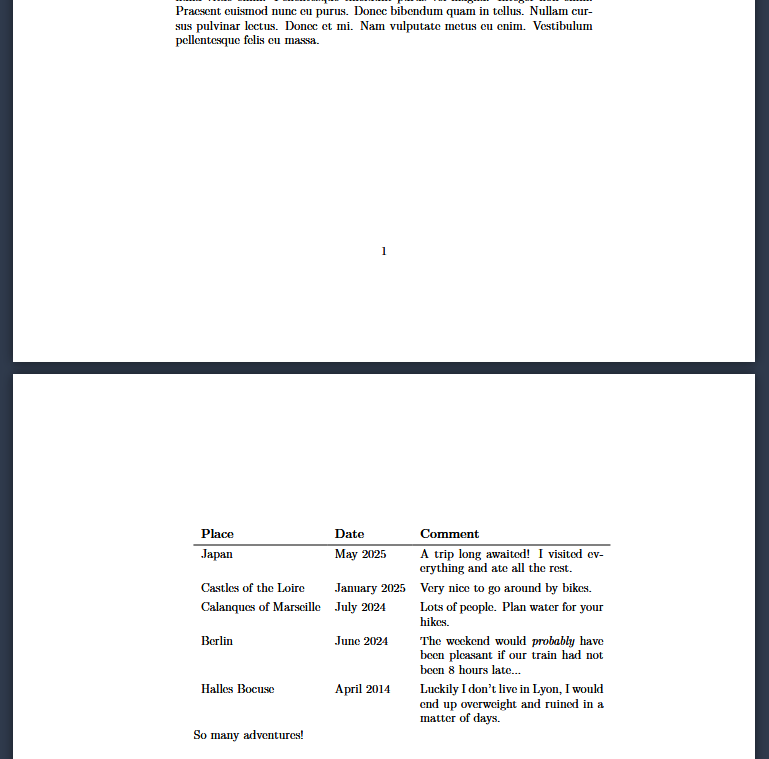
\includegraphics[width=\linewidth]{../img/longtblr_intro2}
\end{center}

Because there is not enough place on the initial page anymore, the table is displayed on the next page and an ugly empty space remains. 

For this reason, it is often better to let Latex decide where the table should be displayed. For this, we signal to Latex to remove the table from the flow of text by passing it to \emph{float mode}. We can also use this as an opportunity to give a caption to our table and a name, that we'll use whenever we want to refer to it.

\begin{Code}
You'll find in Table~\highLight{\ref{table:my-trips}} the list of my previous trips:

\highLight{\begin{table}[htbp]}
	\begin{tblr}{
		colspec = {llX},
		row{1} = {font=\bfseries},
	}
		Place & Date & Comment \\ \hline
	Japan & May 2025 & A trip long awaited! I visited everything and ate all the rest. \\
	Castles of the Loire & January 2025 & Very nice to go around by bikes. \\
	Calanques of Marseille & July 2024 & Lots of people. Plan water for your hikes. \\
	Berlin & June 2024 & The weekend would \textit{probably} have been pleasant if our train had not been 8 hours late...\\
	Halles Bocuse & April 2014 & Luckily I don't live in Lyon, I would end up overweight and ruined in a matter of days.
	\end{tblr}
	\highLight{\caption{All my trips over the last years}\label{table:my-trips}}
\highLight{\end{table}}

So many adventures!
\end{Code}

A few notes:

\begin{itemize}
	\item The environment \snippet{\textbackslash begin\{table\}} and \snippet{\textbackslash end\{table\}} define a floating table. This environment is native from Latex, and does not come from tabularray.
	\item The options \snippet{[htbp]} given to that environment indicate where you would like the table to be, from best desirable outcome to least. Latex will try to make you happy but is sometimes very stubborn about where a table should be. The options stand for:
	\begin{itemize}
		\item \textbf{h}ere: the table is placed where we wrote it in the flow
		\item \textbf{t}op: the table is placed at the top of the current page
		\item \textbf{b}ottom: the table is placed at the bottom of the current page
		\item next \textbf{p}age: the table is placed in the next page.
	\end{itemize}
	\item We added a visible caption with the command \snippet{\textbackslash caption}
	\item We gave a name to the table with the command \snippet{\textbackslash label}, and referred to it with the command \snippet{\textbackslash ref} (you can also use \snippet{\textbackslash cref} if you use the package \snippet{cleveref})
\end{itemize}

\begin{infobox}{TL;DR}
	\begin{itemize}
		\item Use the environment \snippet{\textbackslash begin[htpb]\{table\}} and \snippet{\textbackslash end\{table\}} to transform your table into a float. You can position the float with the options \snippet{h} (here), \snippet{t} (top), \snippet{b} (bottom), \snippet{p} (next page).
		\item Use \snippet{\textbackslash caption} to give a caption to your table, and \snippet{\textbackslash label} to give it a name you can refer to with \snippet{\textbackslash caption}
	\end{itemize}
\end{infobox}